%!TEX root = widefieldscan.tex
\svnidlong
{$HeadURL$}
{$LastChangedDate$}
{$LastChangedRevision$}
{$LastChangedBy$}

\begin{center}
	\fbox{
		\begin{minipage}{.618\textwidth}
		The file of this section is \url{\svnkw{HeadURL}}, was last changed at: \svnfileday.\svnfilemonth.\svnfileyear \space \svnfilehour:\svnfileminute \space (UTC\svnfiletimezone) and is at revision \svnkw{LastChangedRevision}.
		\end{minipage}
	} 
\end{center}

\section{Materials and Methods}
\label{sec:materials and methods}
\subsection{Animal Handling and Tissue Preparation}
The preparation of the lung samples has been performed according to~\citet{Schittny1997,Schittny1998}. Briefly, lungs of Sprague-Dawley rats have been extracted after they have been perfused and filled with phosphate buffered saline by instillation via tracheostomy until the mid respiratory lung volume was reached.

The extracted lung lobes have been fixed for potential storage in 2.5\% glutaraldehyde (C$_5$H$_8$O$_2$). For the preparation of the imaging the samples have been postfixed---comparable to electron microscopy protocols---with \SI{1}{\percent} osmium tetroxide (OsO$_4$) and stained with \SI{4}{\percent} uranyl acetate (C$_4$H$_6$O$_6$U), dehydrated in a graded series of ethanol and transferred into paraffin~\cite{Schittny1998,Schittny1997}\todo{citations (taken from Schittny2008) still valid for our protocol?}. Osmium tetroxide and uranyl acetate exhibit a higher absorption for x-rays than the unstained lung tissue, thus enhancing the contrast of the resulting tomographic images. The lung samples have been mounted onto standard electron microscopy sample mounts with a diameter of approximately \SI{13}{\milli\meter} (PLANO GmbH, Wetzlar, Germany) using paraffin.

Handling of the animals before and during the experiments, as well as the experiments themselves, were approved and supervised by the Swiss Agency for the Environment, Forests and Landscape and the Veterinary Service of the Canton of Bern.

\subsection{SRXTM}
All experiments were performed at the Swiss Light Source, Paul Scherrer Institut, Villigen, Switzerland; at the TOMCAT beamline, which is located at the X02DA port of the SLS and is one of 17 currently operating beamlines. TOMCAT receives photons from a \SI{2.9}{\tesla} super-bending magnet. The critical energy of this super-bending magnet is \SI{11.1}{\kilo\electronvolt} (corresponding to a wavelength of \SI{0.122}{\nano\meter}). A double crystal multilayer monochromator covers an energy range between 6 and \SI{45}{\kilo\electronvolt} with a bandwidth range of a few percent to \SI{e-4}. Detailed technical specifications of the beamline and beam characteristics have been described by~\citeauthor{Stampanoni2006a}~\cite{Stampanoni2006a,Stampanoni2007}.

\subsubsection{Image Acquisition}
\label{seq:Image Acquisition}
The sample holder at TOMCAT is equipped with an appropriate collet chuck to mount standard electron microscopy (EM) sample tables into the beam. The samples have been scanned at an x-ray energy of \SI{12.6}{\kilo\electronvolt}. After penetration of the sample, the x-rays are converted into visible light by a Ce-doped YAG scintillator (Crismatec Saint-Gobain, Nemours, France). The projection images were further magnified by diffraction limited microscope optics and digitized by a high-resolution 2048$\times$2048 pixel CCD camera (PCO AG, Kelheim, Germany) with 14 bit nominal dynamic range which can record projections into the internal memory of \SI{4}{\giga\byte}. All samples were imaged using a 10$\times$ magnification, with 2$\times$2 binning and \SI{125}{\milli\second} exposure time or no binning and \SI{500}{\milli\second} exposure time, resulting in isotropic voxels with a side length of \SI{1.43}{\micro\meter} or \SI{0.72}{\micro\meter}, respectively.

\subsubsection{Generation of tomographic datasets}
The principles of x-ray computed tomography are explained in details by \citet{Kak2002} and \citet{Hsieh2003}. Briefly, projection images $I_{Pr}$---essentially single radiographies---of the sample are recorded at several angular positions between \SI{0}{\degree} and \SI{180}{\degree}. Additionally, a set of dark ($I_{D}$) and flat images ($I_{F}$) are recorded. The dark image set is obtained with a closed shutter at the start of the scan, it captures the camera noise and dark current and is used to baseline correct the projection images. The flat image set is recorded at the start and at the end of the scan, it captures the beam profile and is used to normalize the projection images. The corrected projection images $I_{cPr}$ are then corrected with the average dark ($\overline{I_{D}}$) and average flat image ($\overline{I_{F}}$) using equation~\ref{eq:cpr}.
\begin{equation}
	I_{cPr} = -ln\left(\frac{I_{Pr}-\overline{I_{D}}}{\overline{I_{F}}-\overline{I_{D}}}\right)
	        = ln(\overline{I_{F}}-\overline{I_{D}})-ln(I_{Pr}-\overline{I_{D}})
	\label{eq:cpr}
\end{equation}
The corrected projections are then transformed into so-called sinograms, where the $n$\textsuperscript{th} is composed of the $n$\textsuperscript{th} line of every corrected projection. One sinogram thus contains as many rows as the amount of obtained corrected projections---the angular steps---and as many columns as the width of the projection images. Each sinogram corresponds to one slice of the tomographic dataset. The $n$\textsuperscript{th} slice of the tomographic scan can be reconstructed from the $n$\textsuperscript{th} sinogram using a standard filtered back-projection~\cite{Kak2002,Hsieh2003} or gridrec~\cite{Dowd1999} algorithm. The absorption properties of the sample are encoded by the gray values of the reconstructed dataset. The full work flow from image acquisition to tomographic dataset on the disk contains several steps more, detailed explanations are described by~\citet{Hintermueller2009}.

%\subsection{Image Processing}
%\label{subsec:image processing}
%After the acquisition of the sub-scan projection images, these image sets are corrected with the so called dark field and flat field images. The dark field images are obtained while all the shutters are closed---thus no x-rays are present---and are used for the detection of camera noise and dark current. The flat field images (FI) are obtained with x-ray beam, but without the sample. They are recorded to remove the varying beam profile brightness from the projection images. The projections (PI) are first baseline corrected, then the average of the dark images is subtracted and afterwards they are normalized into corrected projections (CPR) as seen in equation~\ref{eq:correction}:%
% \begin{equation}
%	\text{CPR}=-ln\left(\frac{\text{PI}}{\text{FI}}\right)=ln(\text{FI})-ln(\text{PI})
%	\label{eq:correction}
% \end{equation}

\subsection{Wide Field Scanning}
As mentioned in section~\ref{subsec:enhancing the field of view}, to obtain an enhanced FOV, we need to scan the samples with multiple subscans at varying positions covering the whole sample. To achieve this, we have written a custom MATLAB-script \todo{Script(s) in Appendix?}(MATLAB$^\text{\textregistered}$ 7.6.0.321 (R2008a), The MathWorks, Inc.), where the user is able to input the scanning parameters like desired FOV, detector width, desired overlap between the subscans, magnification and binning. The script then simulates different scanning protocols and calculates the expected reconstruction quality, which is then plotted against the acquisition time. Such a plot is shown in figure~\ref{fig:2008c-qualityplot}.

\begin{figure}
	\centering
		%\documentclass{article}
%\usepackage{tikz,pgfplots}
%\usepackage[pdftex,active,tightpage]{preview}
%\begin{document}
%\begin{preview}
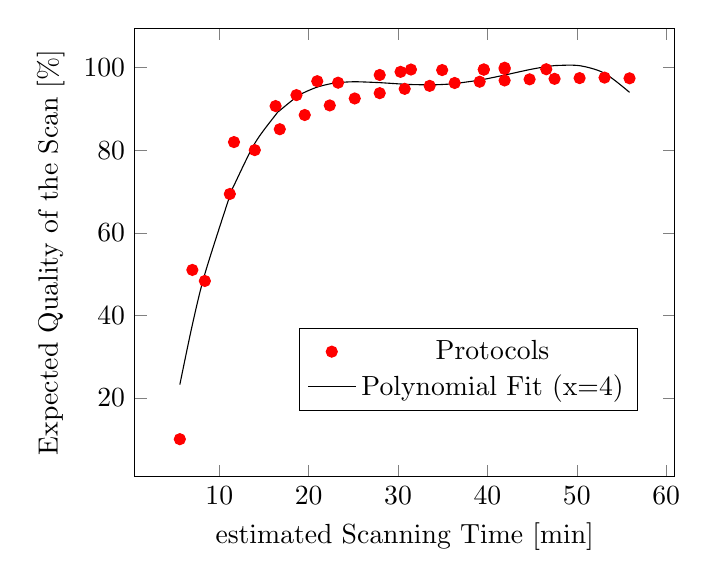
\begin{tikzpicture}
\begin{axis}[%
	xlabel={estimated Scanning Time [min]},%
	ylabel={Expected Quality of the Scan [\%]},%
	]

% Line plot
\addplot [ color = red, only marks, mark = *] 
coordinates{
 (5.5875,10) (6.98958,51.0063) (8.3875,48.3324) (11.1813,69.4075) (11.6458,81.985) (13.975,80.0399) (16.3021,90.7093) (16.7688,85.096) (18.6354,93.3621) (19.5625,88.5423) (20.9625,96.7319) (22.3625,90.8617) (23.2917,96.3704) (25.1563,92.5481) (27.9479,98.2413) (27.95,93.8354) (30.2813,98.9979) (30.7437,94.8773) (31.4438,99.5581) (33.5375,95.6051) (34.9375,99.4314) (36.3375,96.2983) (39.1313,96.6062) (39.5938,99.5875) (39.5958,99.5241) (41.925,100) (41.925,96.9138) (41.9271,99.6929) (44.7188,97.1848) (46.5833,99.6309) (47.5125,97.3067) (50.3125,97.4836) (53.1063,97.603) (55.9,97.4336)
};

% Line plot
\addplot [ smooth ] 
coordinates{
 (5.5875,23.213) (6.98958,37.7379) (8.3875,50.0404) (11.1813,68.9695) (11.6458,71.4736) (13.975,81.6837) (16.3021,88.5733) (16.7688,89.6234) (18.6354,92.9028) (19.5625,94.0559) (20.9625,95.3079) (22.3625,96.078) (23.2917,96.3777) (25.1563,96.6032) (27.9479,96.3862) (27.95,96.3859) (30.2813,96.0569) (30.7437,96.0006) (31.4438,95.9286) (33.5375,95.8484) (34.9375,95.9383) (36.3375,96.1591) (39.1313,96.986) (39.5938,97.167) (39.5958,97.1679) (41.925,98.211) (41.925,98.211) (41.9271,98.212) (44.7188,99.5426) (46.5833,100.268) (47.5125,100.516) (50.3125,100.492) (53.1063,98.6574) (55.9,94.0299)
};


\pgfplotsset{every axis legend/.append style={
at={(0.618,0.2)},
anchor=base}}

\legend{Protocols,Polynomial Fit (x=4)}%$p(x)=p_{1}x^{n}+p_{2}x^{n-1}+...+p_{n}x+p_{n+1}$}

\end{axis}
\end{tikzpicture}
%\end{preview}
%\end{document}
	\caption{Quality-Plot of 34 calculated protocols. The red dots show the expected quality of the different protocols, the black plot is a polynomial fit $p(x)$ with $n=4$ for $p(x)=p_{1}x^{n}+p_{2}x^{n-1}+...+p_{n}x+p_{n+1}$. A subset of 19 protocols have been scanned. Details of these scans are shown in table~\ref{tab:projections} and are discussed in section~\ref{sec:Results}.}
	\label{fig:2008c-qualityplot}
	\todo[inline]{come back to this in results!}
\end{figure}

The proposed protocols are designed in such a way that the total scanning time---which scales with the total amount of recorded projections---can be greatly reduced. Depending on the input of the end-user, we were able to reduce the total acquisition time by \SI{86}{\percent}, as can be seen in table~\ref{tab:projections}. This table provides the details of the 19 different protocols we have scanned of the same sample. This has been done to assess the artifacts which arise through the reduction of the amount of projections. Albeit the aforementioned reduction in scanning time by \SI{86}{\percent} does introduce artifacts in the reconstruction, an automated segmentation of the airways is still possible, as is shown later on.

\begin{table}
\centering
	\caption{Specification of different protocols and time used compared to gold standard}
	\begin{tabular*}{\textwidth}{l@{\extracolsep\fill}ccccccccccccccccccc}
		\toprule
		Protocol 			& B & C & D & E & F & G & H\\
		\midrule
		Total Projections 	& 15732 & 13110 & 13110 & 10925 & 11799 & 9833 & 10488\\
		Time [\%] 			& 100 & 83.33 & 83.33 & 69.44 & 75 & 62.5 & 66.67\\
		\bottomrule
	\end{tabular*}
	\begin{tabular*}{\textwidth}{l@{\extracolsep\fill}ccccccccccccccccccc}
		\toprule
		Protocol 			& I & J & K & L & M & N \\
		\midrule
		Total Projections 	& 5436 & 8740 & 9177 & 7648 & 7866 & 6555 \\
		Time [\%] 			& 34.7 & 55.6 & 58.3 & 48.6 & 50 & 41.7 \\
 		\bottomrule
	\end{tabular*}
	\begin{tabular*}{\textwidth}{l@{\extracolsep\fill}ccccccccccccccccccc}
		\toprule
		Protocol 			& O & P & Q & R & S & T \\
		\midrule
		Total Projections 	& 6555 & 5244 & 4370 & 3933 & 2622 & 2185 \\
		Time [\%] 			& 41.7 & 33.3 & 27.8 & 25 & 16.7 & 13.9 \\
		\bottomrule
	\end{tabular*}
	\label{tab:projections}
\end{table}

After the user has chosen a suitable protocol corresponding to one dot in figure~\ref{fig:2008c-qualityplot}, the MATLAB-script writes a preference file to the disk. This preference file is parsed by a custom Python-script to interact with the EPIC-System (Experimental Physics and Industrial Control System, Argonne National Laboratory, Argonne, USA, \url{http://www.aps.anl.gov/epics/}), which is used to access and control all hardware of the TOMCAT beamline.

We perform several subscans without user intervention, except input of the sample name. All parameters like filename-suffixes of the subscans, sample-position in relation to the beam, rotation angles and amount of projections to obtain for the subscans have been set beforehand by the MATLAB-script, also permitting multiple batch scans of the same sample without any manual intervention. The sample on the sample holder was thus not touched during the acquisition of the 57 different subscans for the 19 mentioned protocols. 

\subsubsection{Covering a broad FOV}
\label{subsec:covering a broad fov}
Generally, tomographic images are obtained in such a manner that the sample is rotated for \SI{180}{\degree} while multiple projection images are obtained, as shown in figure~\ref{fig:covering-one scan}. After reconstructing the sample the width of the image corresponds to the FOV of the camera.

If the sample to be imaged has a size which is slightly larger than the FOV of the camera, a \SI{360}{\degree}-scan is performed. Projections are obtained over a full rotation of the sample, while the sample is positioned in front of the camera in such a way that it only covers half the FOV of the detector. After acquisition of the projection images, half of the dataset has to be flipped and the projections at position $P_{x}$ and $P_{x+\SI{180}{\degree}}$ are stitched together to projection images covering two times the FOV of the camera.

\begin{figure}
	\centering
	\subfloat[\SI{180}{\degree}-scan]{%\documentclass{article}
%\usepackage{tikz}
%\begin{document}

\begin{figure}[tb]
	\centering
	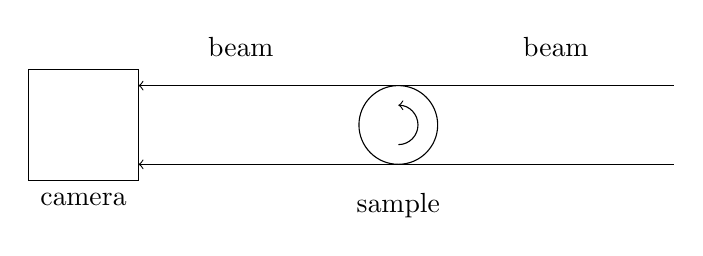
\begin{tikzpicture}
		%drawing grid
		%\draw[color=gray] (0,0) grid (8,1);
		%camera
		\draw (-.2,-.2) rectangle (1.2,1.2);
		\draw (.5,-.25) node [below] {camera};
		% beam
		\draw[<-] (1.2,0) -- (8,0);
		\draw[<-] (1.2,1) -- (8,1);
		\draw (2.5,1.25) node [above] {beam};
		\draw (6.5,1.25) node [above] {beam};
		%sample
		\draw (4.5,0.5) circle (.5);
		\draw (4.5,-.25) node [below] {sample};
		%sample rotation
		\draw[->] (4.5,0.25) arc (-90:90:.25);
	\end{tikzpicture}
	\caption{Covering the FOV -- one scan}
	\label{fig:covering-one scan}
\end{figure}

%\end{document}\label{subfig:cover180}}\\
	\subfloat[\SI{360}{\degree}-scan]{%\documentclass{article}
%\usepackage[pdftex,active,tightpage]{preview}
%\usepackage{tikz}
%\usepackage{pgfplots}
%\usetikzlibrary{plotmarks}
%\begin{document}
%\begin{preview}
	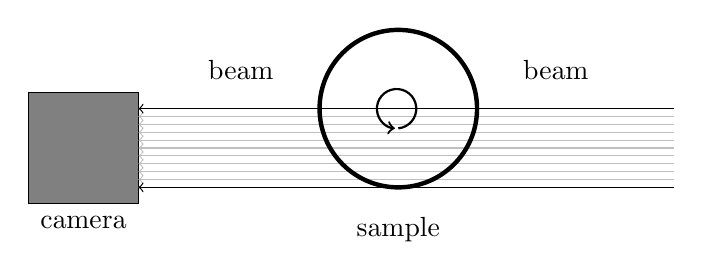
\begin{tikzpicture}
		%drawing grid
		%\draw[color=gray] (0,0) grid (8,1);
		%camera
		\draw[fill=gray] (-.2,-.2) rectangle (1.2,1.2);
		\draw (.5,-.25) node [below] {camera};
		% beam
		\foreach \x in {0,...,10}
			\draw[gray!50,<-] (1.2,0.1*\x) -- (8,0.1*\x);
		\draw[<-] (1.2,0) -- (8,0);
		\draw[<-] (1.2,1) -- (8,1);			
		\draw (2.5,1.25) node [above] {beam};
		\draw (6.5,1.25) node [above] {beam};
		%sample
		\draw[ultra thick] (4.5,1) circle (1);
		\draw (4.5,-.25) node [below] {sample};
		%sample rotation
		\draw[thick,->] (4.5,0.75) arc (-85:265:.25);
	\end{tikzpicture}
%\end{preview}
%\end{document}\label{subfig:cover360}}
	\caption{Covering the FOV of smallish samples with one scan, once for the standard-case and once for the case where the desired FOV is approximately two times bigger than the camera width.}
	\label{fig:covering-one scan}
\end{figure}

\begin{figure}
	\centering
	\documentclass{article}
\usepackage[pdftex,active,tightpage]{preview}
\usepackage{tikz}
\usetikzlibrary{arrows,shapes,backgrounds}
\begin{document}
\begin{preview}
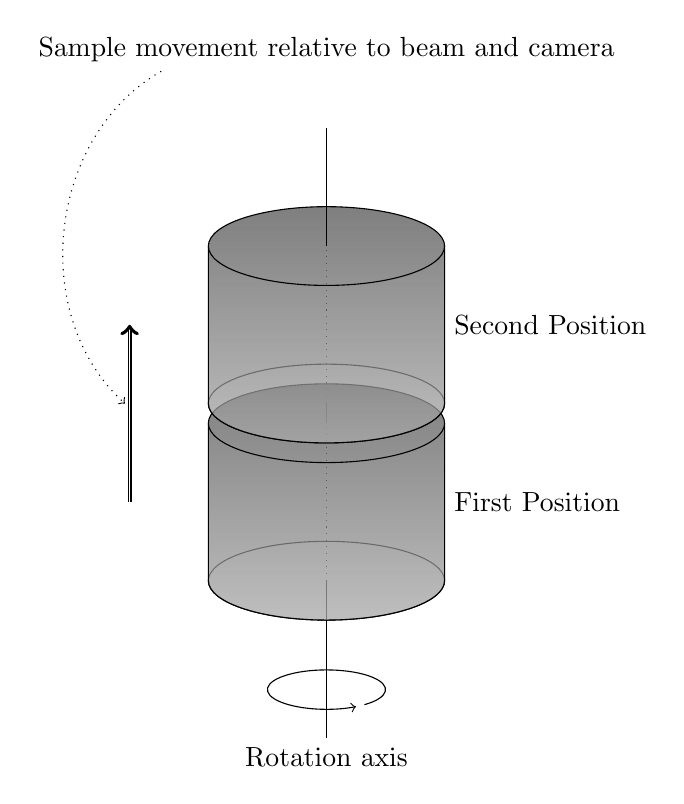
\begin{tikzpicture}%[ultra thick,scale=1]%,show background grid]
	%draw axes
		%\draw[ultra thick] (-10,0) -- (10,0);
		%\draw[ultra thick] (0,-10) -- (0,10);
		%\draw[ultra thick] (0,0) circle (.125);
	% rotation axis
		\draw[->] (0,-2) ++ (-50:.75) arc (-50:300:.75 and .25);
		\draw (0,-3) node [below] {Rotation axis} -- ++(0,2);
		\draw[dotted] (0,-1) -- ++(0,2);
		\draw (0,1) -- ++(0,0.25);
		\draw[dotted] (0,1.25) -- ++(0,2);
	% position 1
		\draw (0,-1) circle (1.5 and .5);
		\fill[shade,semitransparent] (-1.5,-1) arc (-180:0:1.5 and .5) -- ++(0,2) arc (0:180:1.5 and .5) -- cycle;
		\draw (-1.5,-1) arc (-180:0:1.5 and .5) -- ++(0,2) arc (0:180:1.5 and .5) -- cycle;		
		\draw (-1.5,1) arc (-180:0:1.5 and .5);
		\draw (1.5,0) node [right] {First Position};
	% position 2
		\draw (0,1.25) circle (1.5 and .5);
		\fill[shade,semitransparent] (-1.5,1.25) arc (-180:0:1.5 and .5) -- ++(0,2) arc (0:180:1.5 and .5) -- cycle;
		\draw (-1.5,1.25) arc (-180:0:1.5 and .5) -- ++(0,2) arc (0:180:1.5 and .5) -- cycle;		
		\draw (-1.5,3.25) arc (-180:0:1.5 and .5);
		\draw (1.5,2.25) node [right] {Second Position};
	% rotation axis on top
		\draw (0,3.25) -- ++(0,1.5);									
	% sample movement
		\draw[double,->] (-2.5,0) -- (-2.5,2.25) ;% node [text width=10cm,midway,left] {Sample movement relative to beam and camera};	
		% sample movement
		\node (movefrom) at (0,5.75) {Sample movement relative to beam and camera};
		\node (moveto) at (-2.5,1.125) {};
		\draw [->,dotted] (movefrom) to [bend right=54] (moveto);
\end{tikzpicture}
\end{preview}
\end{document}
	\caption{Stacked Scanning - long and thin samples}
	\label{fig:stacked-scanning}
\end{figure}

\begin{figure}
	\centering
	%\documentclass{article}
%\usepackage[pdftex,active,tightpage]{preview}
%\usepackage{tikz}
%\begin{document}
%\begin{preview}
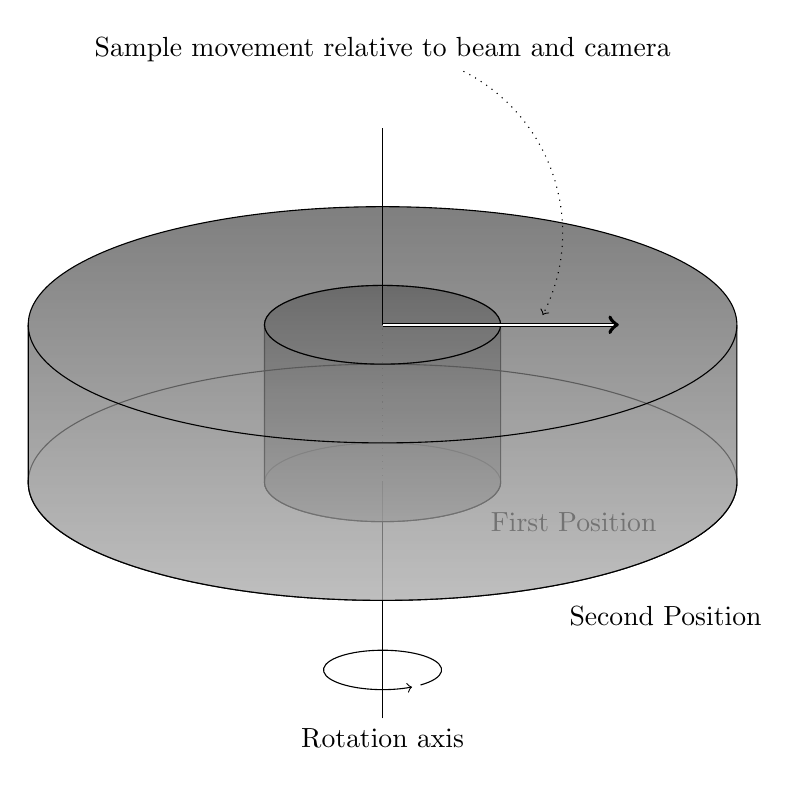
\begin{tikzpicture}%[ultra thick,scale=1]%,show background grid]
	%draw axes
		%\draw[ultra thick] (-10,0) -- (10,0);
		%\draw[ultra thick] (0,-10) -- (0,10);
		%\draw[ultra thick] (0,0) circle (.125);
	% rotation axis
		\draw[->] (0,-3) ++ (-50:.75) arc (-50:300:.75 and .25);
		\draw[] (0,-4) node [below] {Rotation axis} -- ++(0,3);
		\draw[dotted] (0,-1) -- ++(0,2);
	% position 1
		\draw (0,-1) circle (1.5 and .5);
		\fill[shade,semitransparent] (-1.5,-1) arc (-180:0:1.5 and .5) -- ++(0,2) arc (0:180:1.5 and .5) -- cycle;
		\draw (-1.5,-1) arc (-180:0:1.5 and .5) -- ++(0,2) arc (0:180:1.5 and .5) -- cycle;		
		\draw (-1.5,1) arc (-180:0:1.5 and .5);
		\draw (1.25,-1.5) node [right] {First Position};
	% position 2
		\draw (0,-1) circle (4.5 and 1.5);
		\fill[shade,semitransparent] (-4.5,-1) arc (-180:0:4.5 and 1.5) -- ++(0,2) arc (0:180:4.5 and 1.5) -- cycle;
		\draw (-4.5,-1) arc (-180:0:4.5 and 1.5) -- ++(0,2) arc (0:180:4.5 and 1.5) -- cycle;		
		\draw (-4.5,1) arc (-180:0:4.5 and 1.5);
		\draw (2.25,-2.7) node [right] {Second Position};
	% top from position 1 on top
		\draw (0,1) circle (1.5 and .5);
	% rotation axis on top
		\draw (0,1) -- ++(0,2.5);									
	% sample movement
		\draw[double,->] (0,1) -- (3,1);
		\node (movefrom) at (0,4.5) {Sample movement relative to beam and camera};
		\node (moveto) at (2,1) {};
		\draw [->,dotted] (movefrom) to [bend left=45] (moveto);
\end{tikzpicture}
%\end{preview}
%\end{document}
	\caption{Stacked Scanning - broad samples}
	\label{fig:widefield-scanning}
\end{figure}

If we want to achieve tomographic scans covering a sample size which is bigger than what can be achieved with a \SI{360}{\degree}-scan, we have to move the sample in relation to the beam and camera. This can be done as shown in figure~\ref{fig:covering-three scans a}, \todo{which image variant: \ref{fig:covering-three scans a} or \ref{fig:covering-three scans b}?} where we obtain three subscans to be able to reconstruct a FOV covering the whole sample.

\begin{figure}
	\centering
	%\documentclass{article}
%\usepackage[pdftex,active,tightpage]{preview}
%\usepackage{tikz}
%\usepackage{pgfplots}
%\usetikzlibrary{plotmarks}
%\begin{document}
%\begin{preview}
	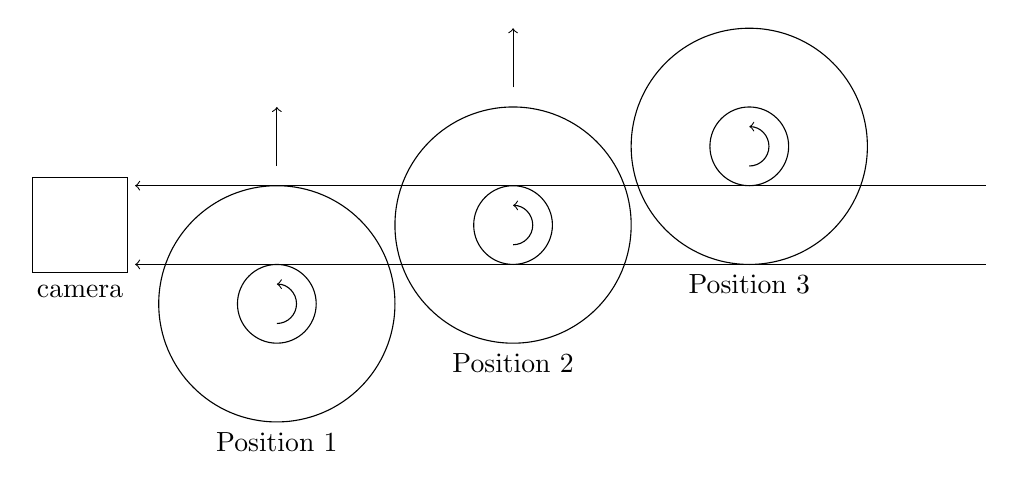
\begin{tikzpicture}[scale=1]
		%drawing grid
%		\draw[color=gray] (0,0) grid (10,1);
		%camera
			\draw (-.1,-.1) rectangle (1.1,1.1);
			\draw (.5,-.35) node {camera};
		% sample positions
			\foreach \x in {1,2,3}{
				\draw     (3*\x,\x-1.5) circle (.5) circle (1.5);			
				\draw[->] (3*\x,\x-1.75) arc (-90:90:.25);
				\draw     (3*\x,-3.25+\x)node {Position \x};
				}
		% movement		
			\foreach \x in {1,2}{				
			    \draw[->]  (3*\x,0.25+\x) -- (3*\x,1+\x);
		% beam
				\draw[<-] (1.2,\x-1) -- (12,\x-1);
				}
	\end{tikzpicture}
%\end{preview}
%\end{document}
	\caption{Covering the FOV -- three scans $\rightarrow$ sample has to move, explain that we still only do \SI{180}{\degree} scans!}
	\label{fig:covering-three scans a}
\end{figure}

\begin{figure}
	\centering
	\documentclass{article}
\usepackage[pdftex,active,tightpage]{preview}
\usepackage{tikz}
\usepackage{pgfplots}
\usetikzlibrary{plotmarks}
\begin{document}
\begin{preview}
%%%%%%%%%%%%%%%%%%%%%%%%%%%%%%%%%
	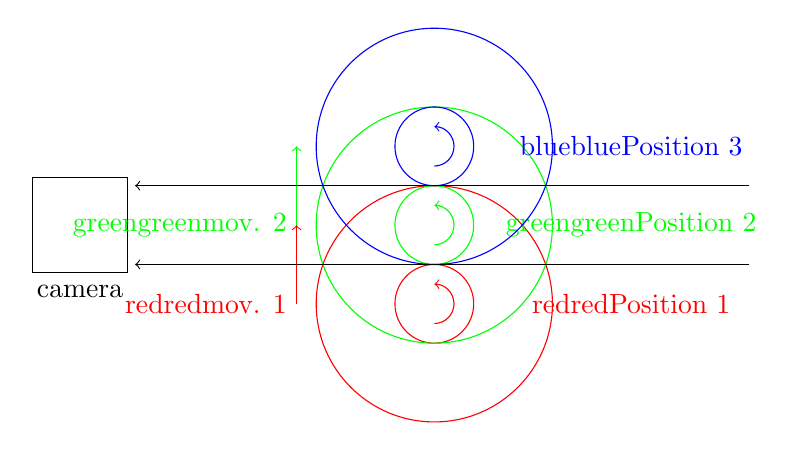
\begin{tikzpicture}
		%camera
			\draw (-.1,-.1) rectangle (1.1,1.1);
			\draw (.5,-.35) node {camera};
		% sample positions
			\foreach \x/\color in {1/red,2/green,3/blue}{
				\draw[color=\color]    (5,\x-1.5) circle (.5) circle (1.5);			
				\draw[color=\color,->] (5,\x-1.75) arc (-90:90:.25);
				\draw[color=\color]    (7.5,\x-1.5) node {Position \x};
				}
		% movement		
			\foreach \x/\e/\color in {1/3.25/red,2/3.25/green}{				
			    \draw[color=\color,->] (\e,-1.5+\x) node [left] {mov. \x} -- (\e,-.5+\x);
			    }
			 \foreach \x in {1,2}{				
		% beam
				\draw[<-] (1.2,\x-1) -- (9,\x-1);
				}
	\end{tikzpicture}
%%%%%%%%%%%%%%%%%%%%%%%%%%%%%%%%%
\end{preview}	
\end{document}
	\caption{Or is this better for the understanding?: Covering the FOV -- three scans $\rightarrow$ sample has to move, explain that we still only do \SI{180}{\degree} scans!}
	\label{fig:covering-three scans b}
\end{figure}

To cover the desired FOV, the projection images have to be obtained in such a manner that they overlap each other slightly. This overlap facilitates the correct stitching of the single projections. Preliminary experiments have shown that even with thorough calibration the combined positioning error of the mechanical setup of TOMCAT is in the order of some pixels. This is an excellent achievement of the whole TOMCAT-team, but for our needs a precision of one pixel is crucial. Obtaining subscans with an overlap of approximately 20 pixels allows us to stitch the subscan projections with a precision of one pixel after having calculated the cutline (as described in section~\ref{sec:Image Merging and Reconstruction}).

After correction with the dark and flat images, the projections of the single overlapping subscans are merged into one projection which covers the full FOV chosen by the user (see figure~\ref{fig:merge-proj}). According to~\citet{Hintermueller2009} the cutting line to remove the overlap is calculated using the mean squared difference between adjacent subscan images. Briefly, for each displacement $\xi_{i,j}$ of the images $i$ and $j$ the mean squared difference of the displacement $\delta^2(\xi_{i,j})$ is computed. This displacement measure provides a measure for the inequality of the two images within their overlapping parts. The local minimum of $\delta^2(\xi_{i,j})$ shows the effective displacement $\xi_{i,j}$ between the two adjacent images $i$ and $j$. For three subscans we calculate the effective displacement $\xi_{1,2}$ and $\xi_{2,3}$ and stitch all the images into one big projection image.

To fulfill the sampling theorem as defined in section~\ref{subsec:enhancing the field of view}, different amount of projections ($N_{i}$) have been recorded for each subscan $i$---at the lateral positions we record more projections compared to the central position. The stitching algorithm thus has to selectively stitch projections from subscan 1 with several projections from subscan 2 and 3 to one projection covering the combined FOV.

Figure \ref{fig:amount of projections} shows how projections from the different subscans relate to each other. Here we describe the most simple case, where the user has chosen a scanning protocol where the sampling theorem is completely fulfilled, thus we record 180 projections for the central and two times 360 projections for the two ring-scans. We have implemented a simple strategy for designing the different protocols; to facilitate the merging of the projections from each subscan, the amount of projections from the inner to the outer subscans is always dividable by two: 
\begin{equation}
	\frac{P_{outer}}{P_{inner}} \bmod 2 = 0
\label{eq:Modulo}
\end{equation}
This approach facilitates the merging of the different subscans in such a way that we can stitch several projections from the inner subscan with projections from the outer subscan as shown in figure~\ref{fig:amount of projections}.

\begin{figure}
	\centering
	%\documentclass{minimal}
%\usepackage[pdftex,active,tightpage]{preview}
%\usepackage{tikz}
%\begin{document}
%\begin{preview}
%\begin{center}
%%%%%%%%%%%%%%%%%%%%%%%%%%%%%	
	\def\radius{1}
	\def\shift{.3}
	\def\overlap{.075}
	\begin{tikzpicture}[scale=1.5]
		%% inner ring
		\draw (0,0) circle (\radius);
		\foreach \angle / \label in 
			{0,20,...,181}
			{
				\draw (\angle:-\radius) -- (\angle:\radius+\shift);
				\draw (\angle:\radius+1.618*\shift) node{\textsf{\label}};
			}
		\foreach \angle in 
			{0,2,...,180}
			{
				\draw (\angle:\radius-.5*\shift) -- (\angle:\radius+.5*\shift);
			}
		%% outer ring			
		\draw (0,0) circle (3*\radius);
		\foreach \angle / \label in 
			{0,20,...,719}
			{
				\draw (.5*\angle:\radius) -- (.5*\angle:3*\radius+\shift);
				\draw (.5*\angle:3*\radius+1.618*\shift) node{\textsf{\label}};
			}
		\foreach \angle in 
			{0,1,...,359}
			{
				\draw (\angle:3*\radius-.5*\shift) -- (\angle:3*\radius+.5*\shift);
			}
		\def\projangle{17}			
		%% RingScan 1
		\draw [ultra thick,color=red](\projangle:\radius-\overlap) -- (\projangle:3*\radius);
		\fill [color=red,nearly transparent] (1,0) -- (3,0) arc (0:180:3*\radius) -- (-1+\overlap,0) arc (180:0:\radius-\overlap);
		%% Central Scan
		\draw [ultra thick,color=green](\projangle+180+2:\radius+\overlap) -- (\projangle+2:\radius+\overlap);
		\fill [color=green,nearly transparent] (0,0) circle (\radius+\overlap);
		%% Ringscan 2
		\draw [ultra thick,color=blue](\projangle+180:3*\radius) -- (\projangle+180:\radius-\overlap);
		\fill [color=blue,nearly transparent] (1,0) -- (3,0) arc (0:-180:3*\radius) -- (-1+\overlap,0) arc (-180:0:\radius-\overlap);
	\end{tikzpicture}%
%%%%%%%%%%%%%%%%%%%%%%%%%%%%%	
%\end{center}
%\end{preview}
%\end{document}%
	\caption{Number of merged projections for one central- and two ring-scan. We assume that we have obtained 180 projections for the central scan and thus acquire two times 360 projections for the lateral scans. This enables us to stitch the projections $P_{1_{34}}$ (red line) from subscan 1 (red area), projection $P_{2_{17}}$ (green line) from the central subscan 2 (green area) and projection $P_{3_{394}}$ (blue line) of subscan 3 (blue area) to one big projection $P_{merge_{34}}$ which covers the full FOV. The areas of the three subscans overlap slightly as described above to account for variations in positioning. For didactic reasons we shifted the central projection (green) by \SI{2}{\degree}, or else the overlap between these particular projection would not be visible.}%
	\todo[inline]{Do we only speak of central and ring-scan or of 3 subscans?}
	\label{fig:amount of projections}%
\end{figure}

%\begin{figure}
%	\centering
%	%\documentclass{minimal}
%\usepackage[pdftex,active,tightpage]{preview}
%\usepackage{tikz}
%\begin{document}
%\begin{preview}
%%%%%%%%%%%%%%%%%%%%%%%%%%%%%
	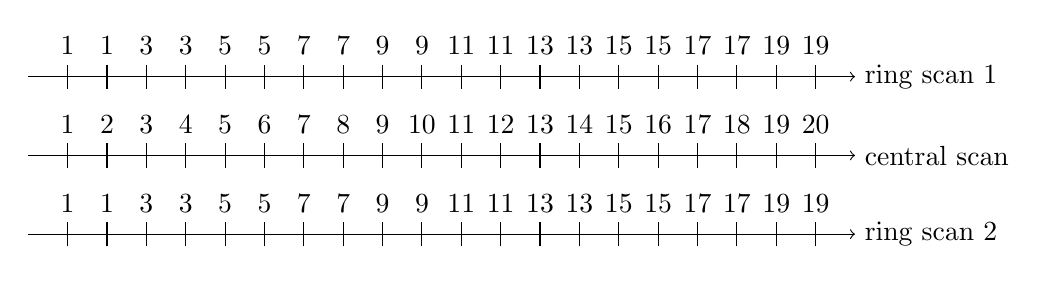
\begin{tikzpicture}[scale=0.5]
	%
	\def\linegap{2}%1.6181229773462783171521035598706}
	\def\length{20}
	\def\ticklength{.309}
	%
	\foreach \y/\label in {0/central scan,\linegap/ring scan 1,-\linegap/ring scan 2}%
		\draw [->] (0,\y) -- (\length+1,\y) node [anchor=west] {\label} ;
	\foreach \x in {1,...,\length}
		\draw (\x,0-\ticklength) -- (\x,0+\ticklength) node [anchor=south] {\x};
	\foreach \z in {1,3,...,\length}
		\draw (\z,\linegap-\ticklength) -- (\z,\linegap+\ticklength) node [anchor=south] {\z}
		(\z+1,\linegap-\ticklength) -- (\z+1,\linegap+\ticklength) node [anchor=south] {\z};
	\foreach \z in {1,3,...,\length}
		\draw (\z,-\linegap-\ticklength) -- (\z,-\linegap+\ticklength) node [anchor=south] {\z}
		(\z+1,-\linegap-\ticklength) -- (\z+1,-\linegap+\ticklength) node [anchor=south] {\z};
	\end{tikzpicture}
%%%%%%%%%%%%%%%%%%%%%%%%%%%%%
%\end{preview}
%\end{document}
%
%	\caption{Number of merged projections for one central- and two ring-scan. Linear variant. The numbers above the ticks denote the number of the projection. Projections vertically above each other will be merged.}%
%	\label{fig:amount of projections - linear}%
%\end{figure}

\subsubsection{Merging and Reconstruction}
All steps mentioned above have been implemented in a set of custom MATLAB functions and scripts which take the parameters of the single subscans (e.g.\ sample name, amount of subscans, amount of dark and flat images) and desired output-name and -suffix as inputs and performs all necessary calculations like loading, normalizing, interpolation and correct stitching of the images into wide field projections. Exemplary results can be seen in figure~\ref{fig:subscans} and \ref{fig:merge-proj}.

After the merging of the normalized projections, the merged projections were reconstructed into the virtual tomography slices using a standard filtered back-projection algorithm or a FFT-based gridrec algorithm on a 20-node server farm (Pentium 4, 2.8 GHz processor, 512 MB RAM\todo{cluster node specs?}). This reconstruction results in an image stack of 1024 or 2048 image slices---depending on the binning---in tiff-format.

The reconstructions used for the assessment of the image quality of the 19 different scanned protocols of the same sample show a three-fold (2.93$\times$) increase in FOV from 1024$\times$1024 pixels to 2996$\times$2996 pixels. As a proof of concept, we also scanned and reconstructed a lung sample with 5 subscans, which led to a roughly five-fold (4.74$\times$) increase in available FOV from 2048$\times$2048 pixels to 9703$\times$9703 pixels (see figure~\ref{fig:LungSlabSophie}).
